\subsubsection{Varying partition, source and destination sizes, keeping the same source to destination ratio}

In this experiment we vary the number of sources and destinations, together with total number of nodes, while keeping a constant ratio of 1:8 between the number of sources and destination nodes. We increase the total number of nodes P from 512 to 4096, The first P/16 nodes send data to the last P/2 nodes. Each source has 8 destinations e.g. node 0 sends data to nodes P/2, P/2+1, ... P/2+7. We present results for {\em disjoint}, {\em overlap} and {\em subset} communications using OPTIQ Optimization (OPT), OPTIQ Heuristic (HEU) and MPI\_Alltoallv (MPI). We use 1 MPI/PAMI rank/node. The data size is 8 MB per source-destination pair. 
%We set the $maxload$ to 16 for the Heuristic approach. %already mentioned 

Figure \ref{fig:constantr} shows the throughput for OPT, HEU and MPI. As shown in the figure, the Optimization approach has the highest throughput, followed by the Heuristic approach and MPI\_Alltoallv. This is because OPT and HEU uses multiple paths for data transfer. Additionally, OPT globally balances load for all source-destination pairs. %TODO: We see improved throughput for 4096 nodes in the case of OPT and HEU because ..... data / hopbytes for 512 vs 4096 performance.  

\begin{figure*}[!htbp]
        \centering
        \begin{subfigure}[b]{0.32\textwidth}
                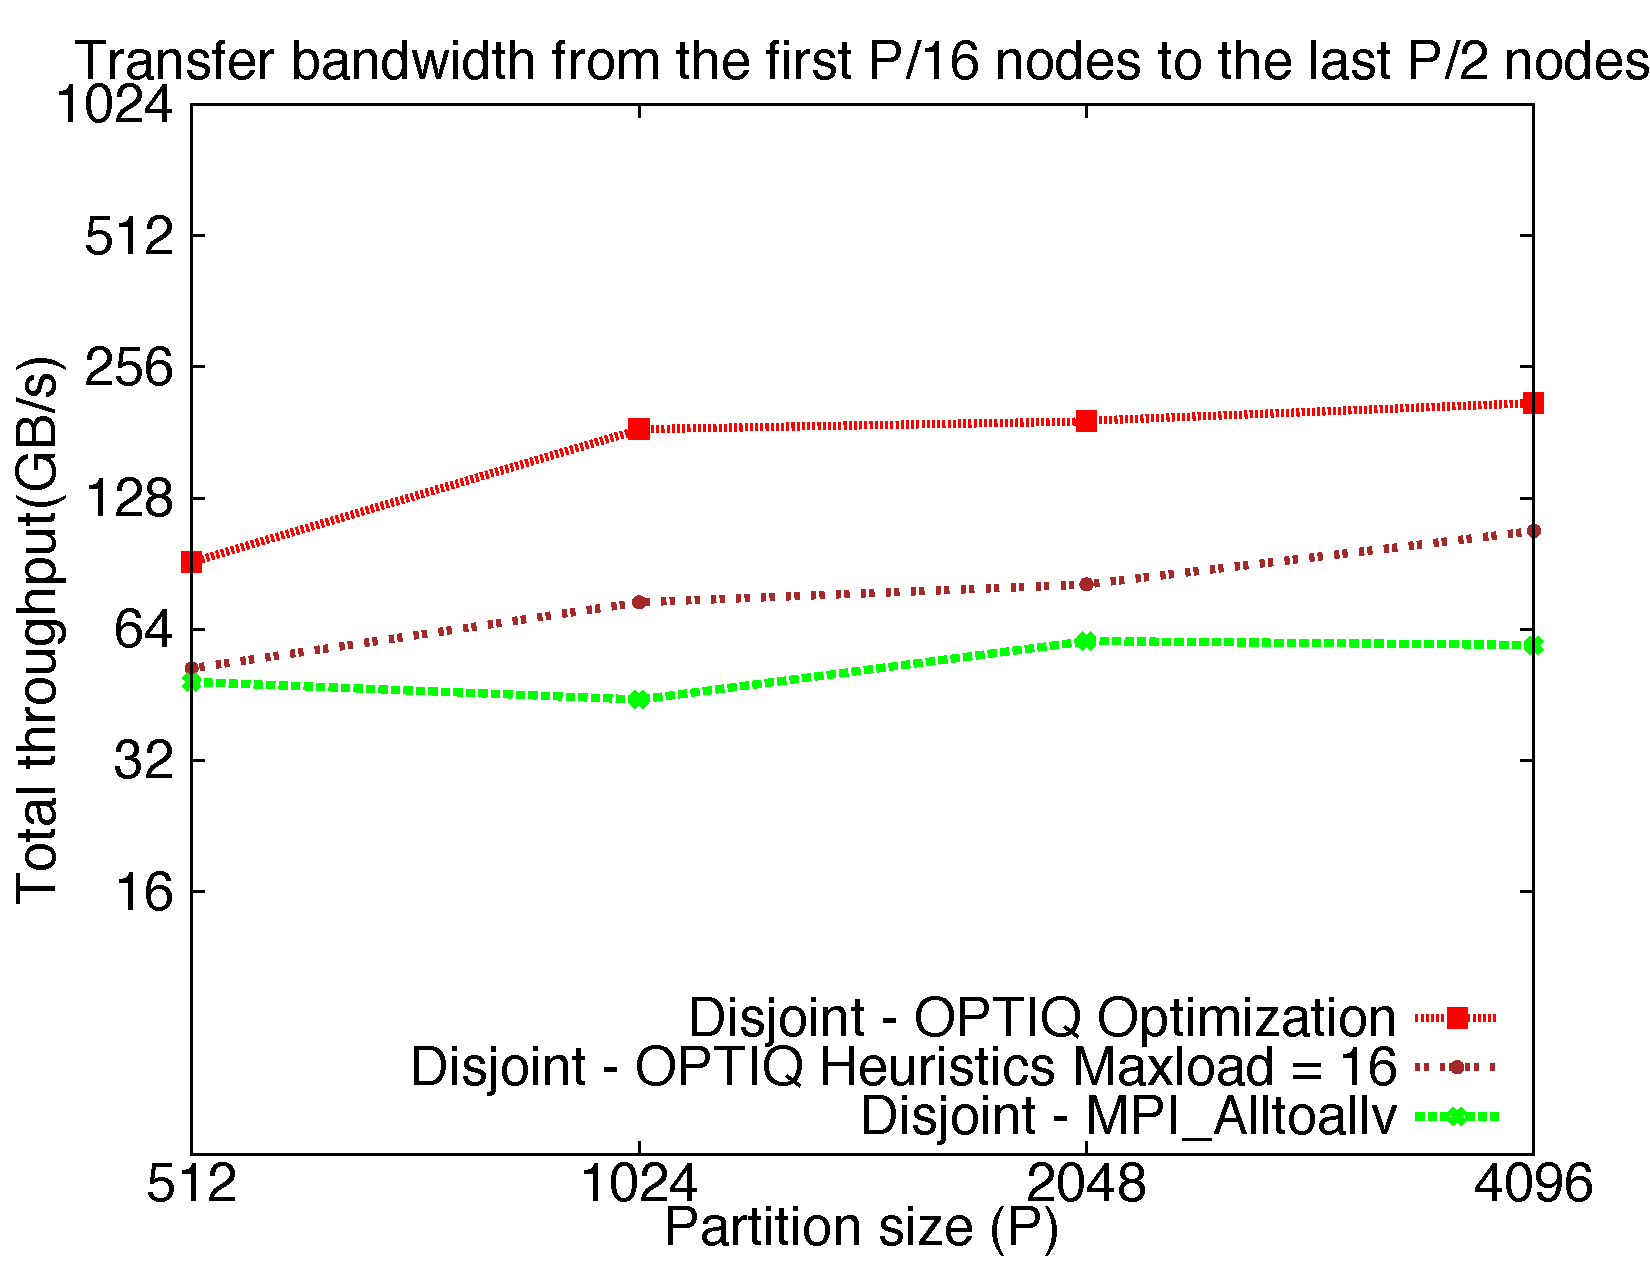
\includegraphics[width=\textwidth]{figures/constantr_3.pdf}
                \caption{Disjoint}
                \label{fig:constantr_3}
        \end{subfigure}%
        ~ %add desired spacing between images, e. g. ~, \quad, \qquad, \hfill etc.
          %(or a blank line to force the subfigure onto a new line)
        \begin{subfigure}[b]{0.32\textwidth}
                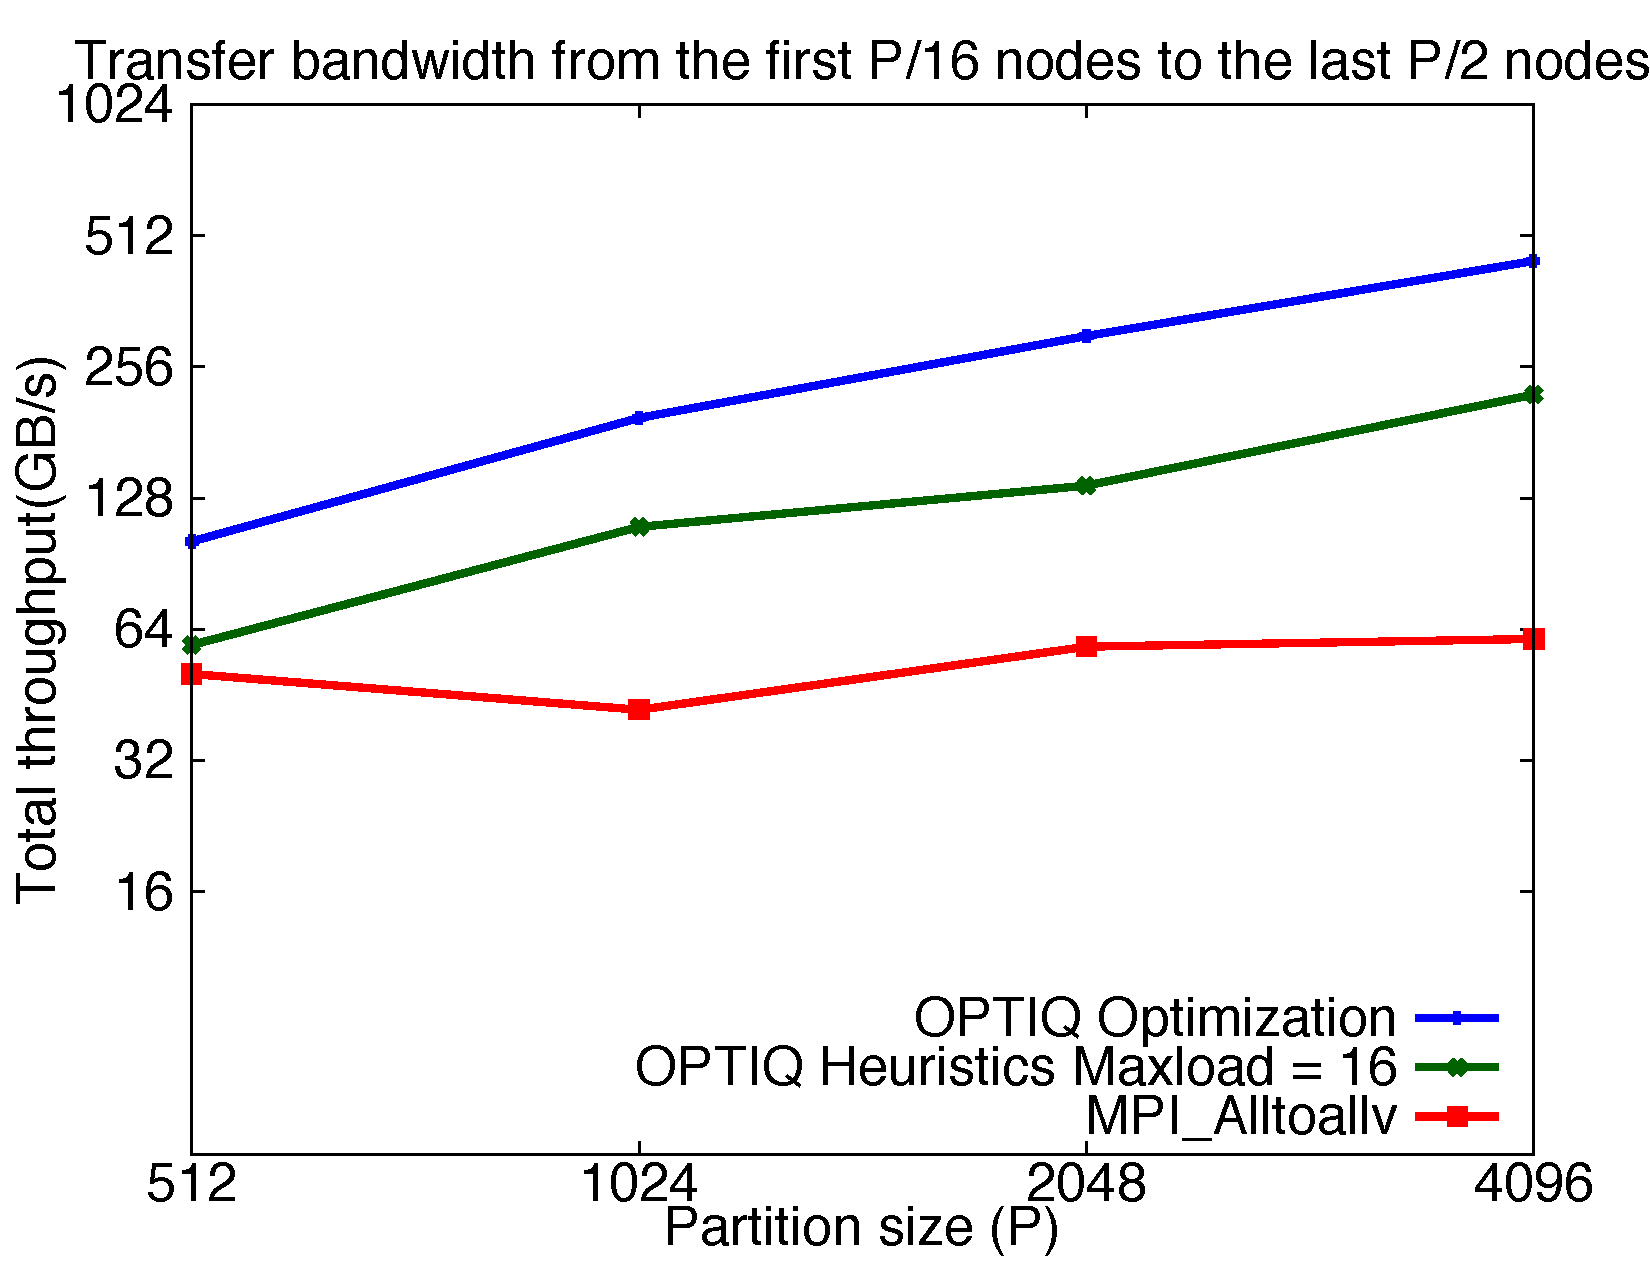
\includegraphics[width=\textwidth]{figures/constantr_27}
                \caption{Overlap}
                \label{fig:constantr_27}
        \end{subfigure}
        ~ %add desired spacing between images, e. g. ~, \quad, \qquad, \hfill etc.
          %(or a blank line to force the subfigure onto a new line)
        \begin{subfigure}[b]{0.32\textwidth}
                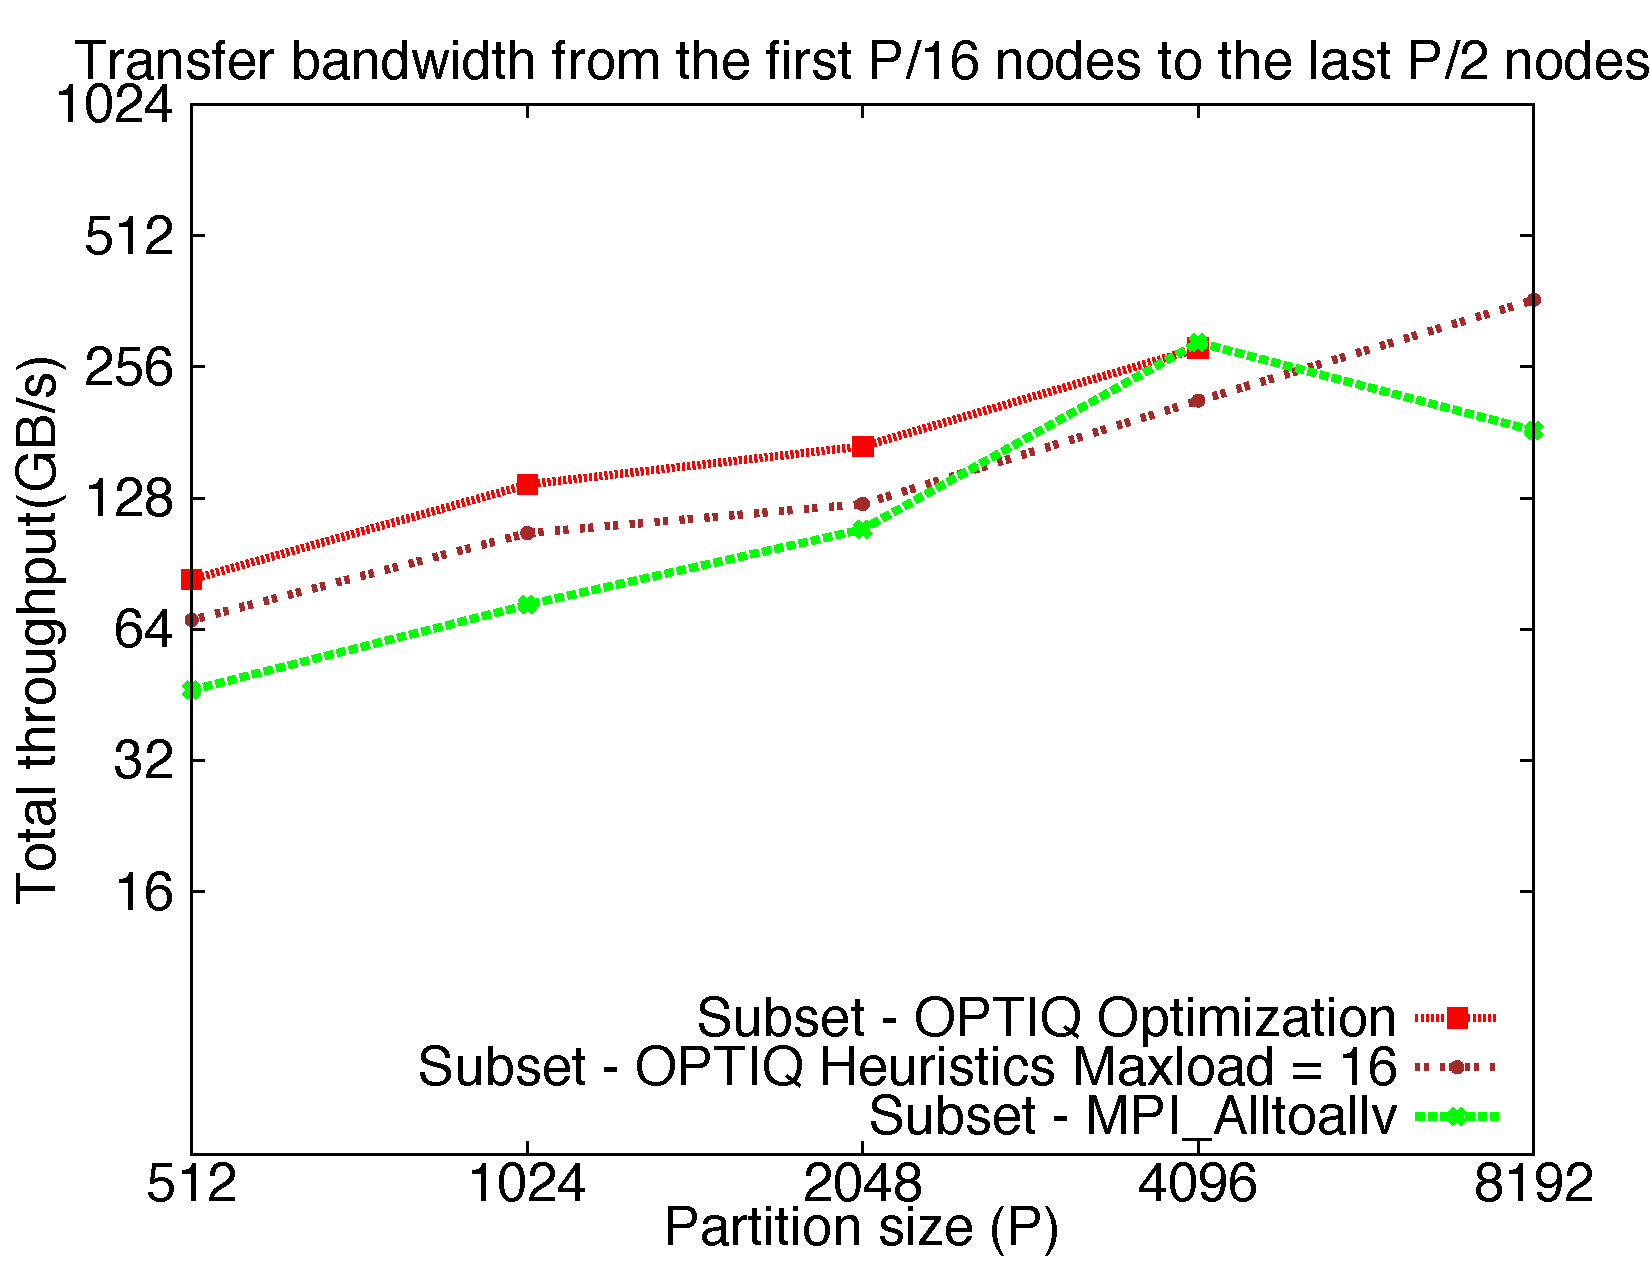
\includegraphics[width=\textwidth]{figures/constantr_87}
                \caption{Subset}
                \label{fig:constantr_87}
        \end{subfigure}
        \caption{Varying the number of sources and destinations and total number of nodes while keeping the ratio constant (1:8).}
	\vspace{-0.15in}
        \label{fig:constantr}
\end{figure*}

Table \ref{table:constantr} shows the throughput, total number of paths per job, the hopbytes per path, the number of copies per path, number of paths per physical link and the total data per link for 1024 nodes. In all three cases, our greedy heuristic is able to find the highest number of paths for the entire data flow. HEU also has the highest maximum and average number of paths per job. However, the paths found by Heuristic are based on local optimization of load on the physical links, as explained in Section~\ref{sec:heuristic}. Therefore, there are higher number of paths per physical link, and higher amount of data per physical link in HEU as compared to OPT. OPT has lower number of paths per link because OPT globally load balances the data transfer on physical links.
%TODO: table remove columns
\begin{comment}
\begin{table*}[!htbp]
   \centering
    \begin{tabular}{| p{0.5cm} | l | r | r | p{0.5cm} | p{0.5cm} | p{0.5cm} | p{0.5cm} |p{0.4cm} | p{0.5cm} |p{0.4cm} | p{0.4cm} |p{0.50cm} | p{0.6cm} |}
    \hline
    \multirow{3}{*}{Pattern} & \multirow{3}{*}{Type} & \multirow{3}{1cm}{BW (GB/s)} & \multicolumn{3}{ c| }{Num. of Paths} & \multicolumn{2}{ c| }{Hopbytes} & \multicolumn{2}{ c| }{Num of copies}& \multicolumn{2}{ c| }{Num of paths} & \multicolumn{2}{ c| }{Total data} \\ \cline{4-6}
    & & & \multirow{2}{0.5cm}{Total Paths} & \multicolumn{2}{ c| }{Per Job} & \multicolumn{2}{ c| }{Per Path (MB)} & \multicolumn{2}{ c| }{Per Path}& \multicolumn{2}{ c| }{Per Link}& \multicolumn{2}{ c| }{Per Link (MB)} \\ \cline{5-14}
    & & & & {Max} & Avg & Max & Avg & Max & Avg & Max & Avg & Max & Avg\\ \hline
    \multirow{3}{*}{Disjont} & OPT    & 188.62 & 1169 & 6 & 2.28 & 83.88 & 23.02 & 1152 & 295.22 & 11 & 2.53 & 18.28 & 9.26 \\ \cline{2-14}
    & HEU & 74.88  & 3146 & 23 & 6.14 & 83.88 & 8.45 & 1152 & 108.24 & 16 & 4.94 & 63.04 & 6.92 \\ \cline{2-14}
    & MPI    & 45.18  & 512  & 1 & 1.00 & 92.27 & 50.33 & & & 16 & 3.07 & 134.21 & 25.76\\ \hline
    \multirow{3}{*}{Overlap} & OPT    & 200.03 & 1303 & 6 & 2.54 & 83.88 & 19.28  & 1152 & 243.96 & 13 & 2.74 & 16.97 & 9.04\\ \cline{2-14}
    & HEU & 113.17  & 3273 & 26 & 6.39 & 75.49 & 7.41 & 1024 & 93.07 & 16 & 5.17 & 38.66 & 7.04 \\ \cline{2-14}
    & MPI    & 42.84 & 512 & 1 & 1.00 & 83.88 & 42.99 &  & & 16 & 3.38 & 134.21 & 28.36 \\ \hline
    \multirow{3}{*}{Subset} & OPT    & 199.20 & 1269 & 6 & 2.48 & 75.49 & 19.48 & 1024 & 245.66 & 11 & 2.79 & 17.10 & 9.32 \\ \cline{2-14}
    & HEU &  61.71 & 3238 & 26 & 6.32 & 75.49 & 7.43 & 1024 & 93.22 & 16 & 5.28 & 45.08  & 7.35 \\ \cline{2-14}
    & MPI    &  41.37 & 512  & 1 & 1.00 & 83.88 &  41.94 & & & 16 & 3.52 & 134.21 & 29.49 \\ \hline
    \end{tabular}
    \caption{Throughput, total number of paths, number of paths per job, maximum and average values of hopbytes, number of copies, number of paths per link and amount of data per link for 3 patterns in 1024 nodes experiments.}
    \label{table:constantr}
\end{table*}
\end{comment}

\begin{table}[!htbp]
   \centering
    \begin{tabular}{| l | l | R{0.6cm} | r | R{0.3cm} | R{0.4cm} | R{0.4cm} | R{0.4cm} | r |}
    \hline
    \multirow{3}{*}{Pattern} & \multirow{3}{*}{Type} & \multirow{3}{1cm}{BW (GB/s)} & \multicolumn{3}{ c| }{Num. of Paths} & \multicolumn{2}{ c| }{Num of paths} & \multirow{3}{1.15cm}{Max amt. of data / link (MB)} \\ \cline{4-6}
    & & & \multirow{2}{0.5cm}{Total Paths} & \multicolumn{2}{ c| }{Per Job} & \multicolumn{2}{ c| }{Per Link}& \\ \cline{5-8}
    & & & & {Max} & Avg & Max & Avg & \\ \hline
    \multirow{3}{*}{Disjont} & OPT    & 188.62 & 1169 & 6 & 2.28 & 11 & 2.53 & 18.28 \\ \cline{2-9}
    & HEU & 74.88  & 3146 & 23 & 6.14 & 16 & 4.94 & 63.04 \\ \cline{2-9}
    & MPI    & 45.18  & 512  & 1 & 1.00 & 16 & 3.07 & 134.21 \\ \hline
    \multirow{3}{*}{Overlap} & OPT    & 200.03 & 1303 & 6 & 2.54 & 13 & 2.74 & 16.97 \\ \cline{2-9}
    & HEU & 113.17  & 3273 & 26 & 6.39 & 16 & 5.17 & 38.66 \\ \cline{2-9}
    & MPI    & 42.84 & 512 & 1 & 1.00 & 16 & 3.38 & 134.21 \\ \hline
    \multirow{3}{*}{Subset} & OPT    & 199.20 & 1269 & 6 & 2.48 & 11 & 2.79 & 17.10 \\ \cline{2-9}
    & HEU &  61.71 & 3238 & 26 & 6.32 & 16 & 5.28 & 45.08 \\ \cline{2-9}
    & MPI    &  41.37 & 512  & 1 & 1.00 & 16 & 3.52 & 134.21 \\ \hline
    \end{tabular}
    \caption{Throughput, total number of paths, number of paths per job, maximum and average values number of paths per link and max amount of data per link for 3 patterns in 1024 nodes experiments.}
    \vspace{-0.15in}
    \label{table:constantr}
\end{table}

Figure \ref{fig:loaddata_histo} shows the distribution of data per link for OPT, HEU and MPI. Optimization approach considers the global load on the network and hence data is distributed among the paths in a more balanced way such that the physical links are load-balanced. Thus, OPT has the lowest maximum amount of data per physical link as shown in Figure \ref{fig:loaddata_histo}. MPI\_Alltoallv has the lowest number of paths. With 1 path per pair of communication, entire data is transferred using the single path, without utilizing the other idle links. %Thus it has the highest hopbytes per path as can be observed in Figure \ref{fig:hopbyte_histo}. 
MPI has the highest amount of data per physical link as can be observed in Figure \ref{fig:loaddata_histo}. Thus MPI has the lowest throughput.
\begin{figure}[!htb]
\vspace{-0.15in}
\centering
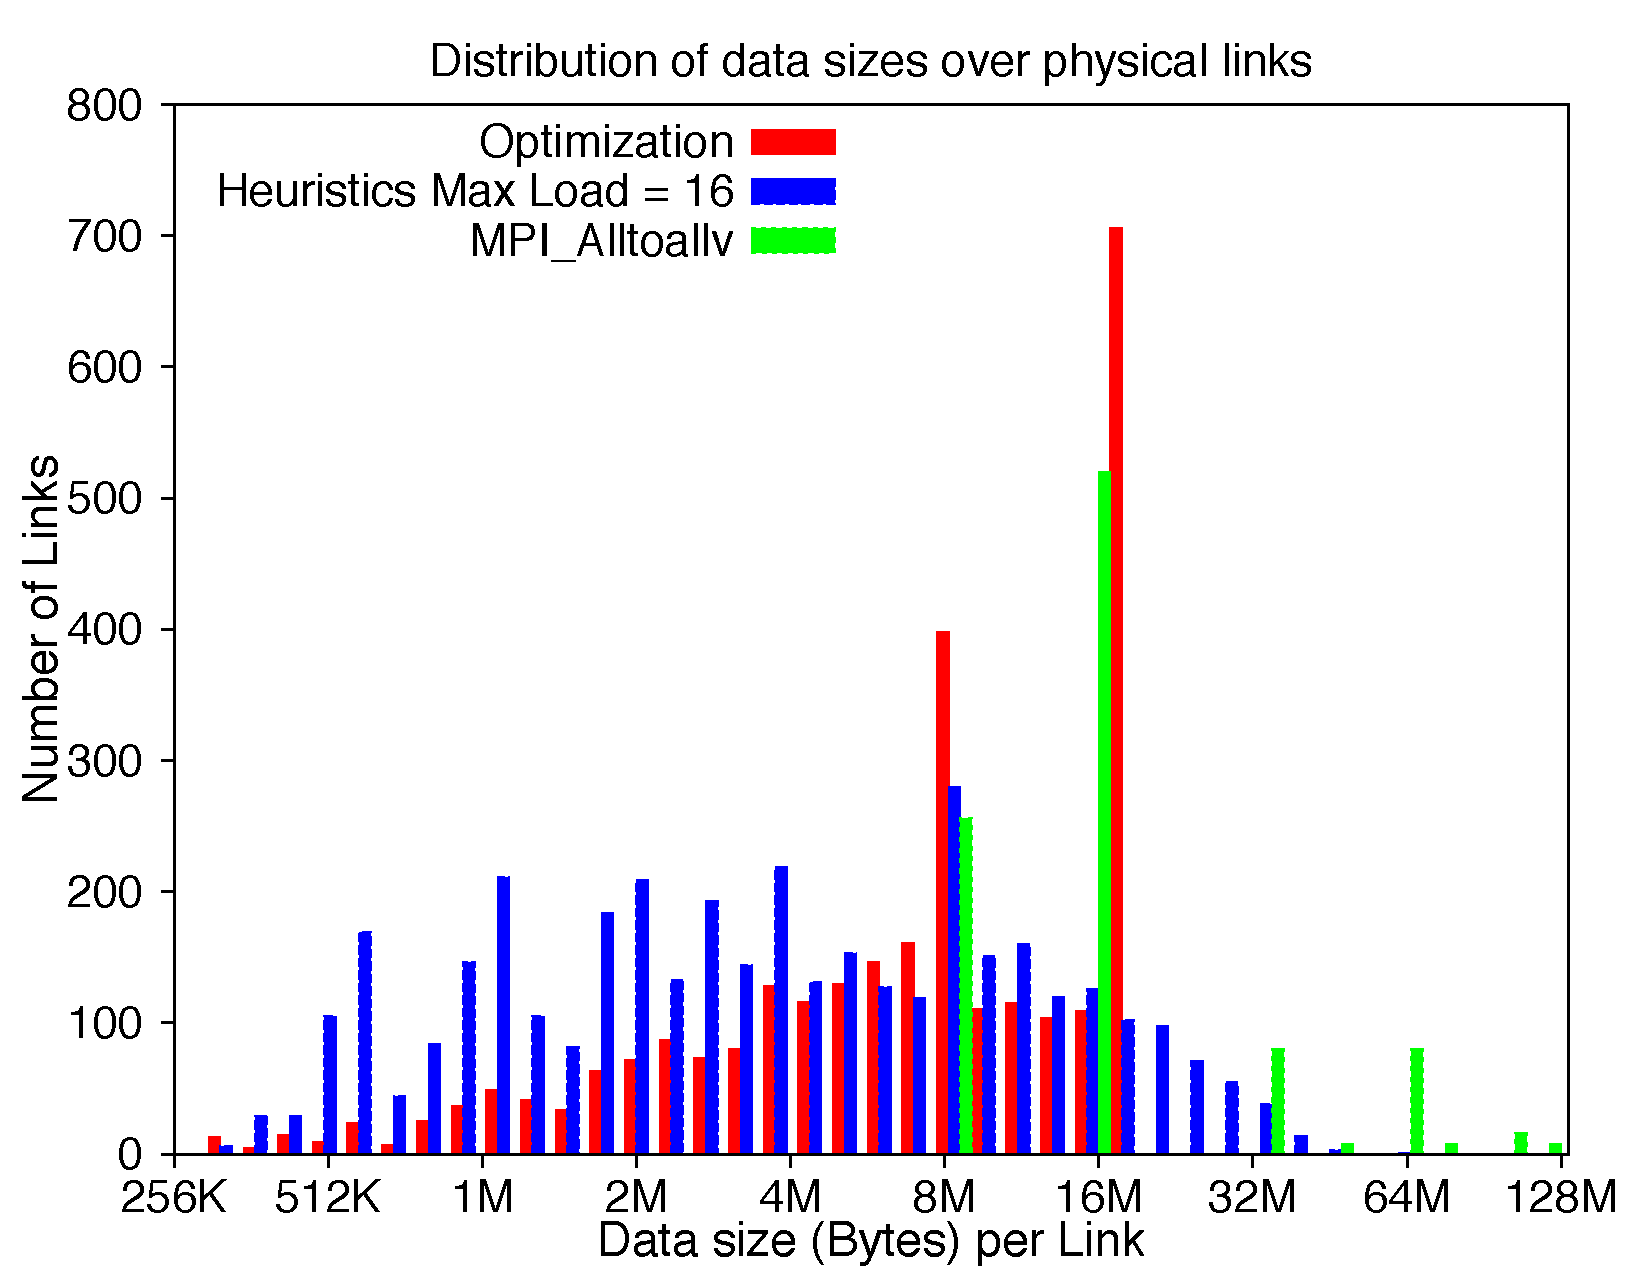
\includegraphics[scale=0.27]{figures/loaddata_histo.pdf}
\vspace{-0.15in}
\caption{Distribution of total amount of data per link for Disjoint pattern in 1024-node partition.}
\vspace{-0.15in}
\label{fig:loaddata_histo}
\end{figure}

%\begin{figure}[!htb]
%\vspace{-0.1in}
%\centering
%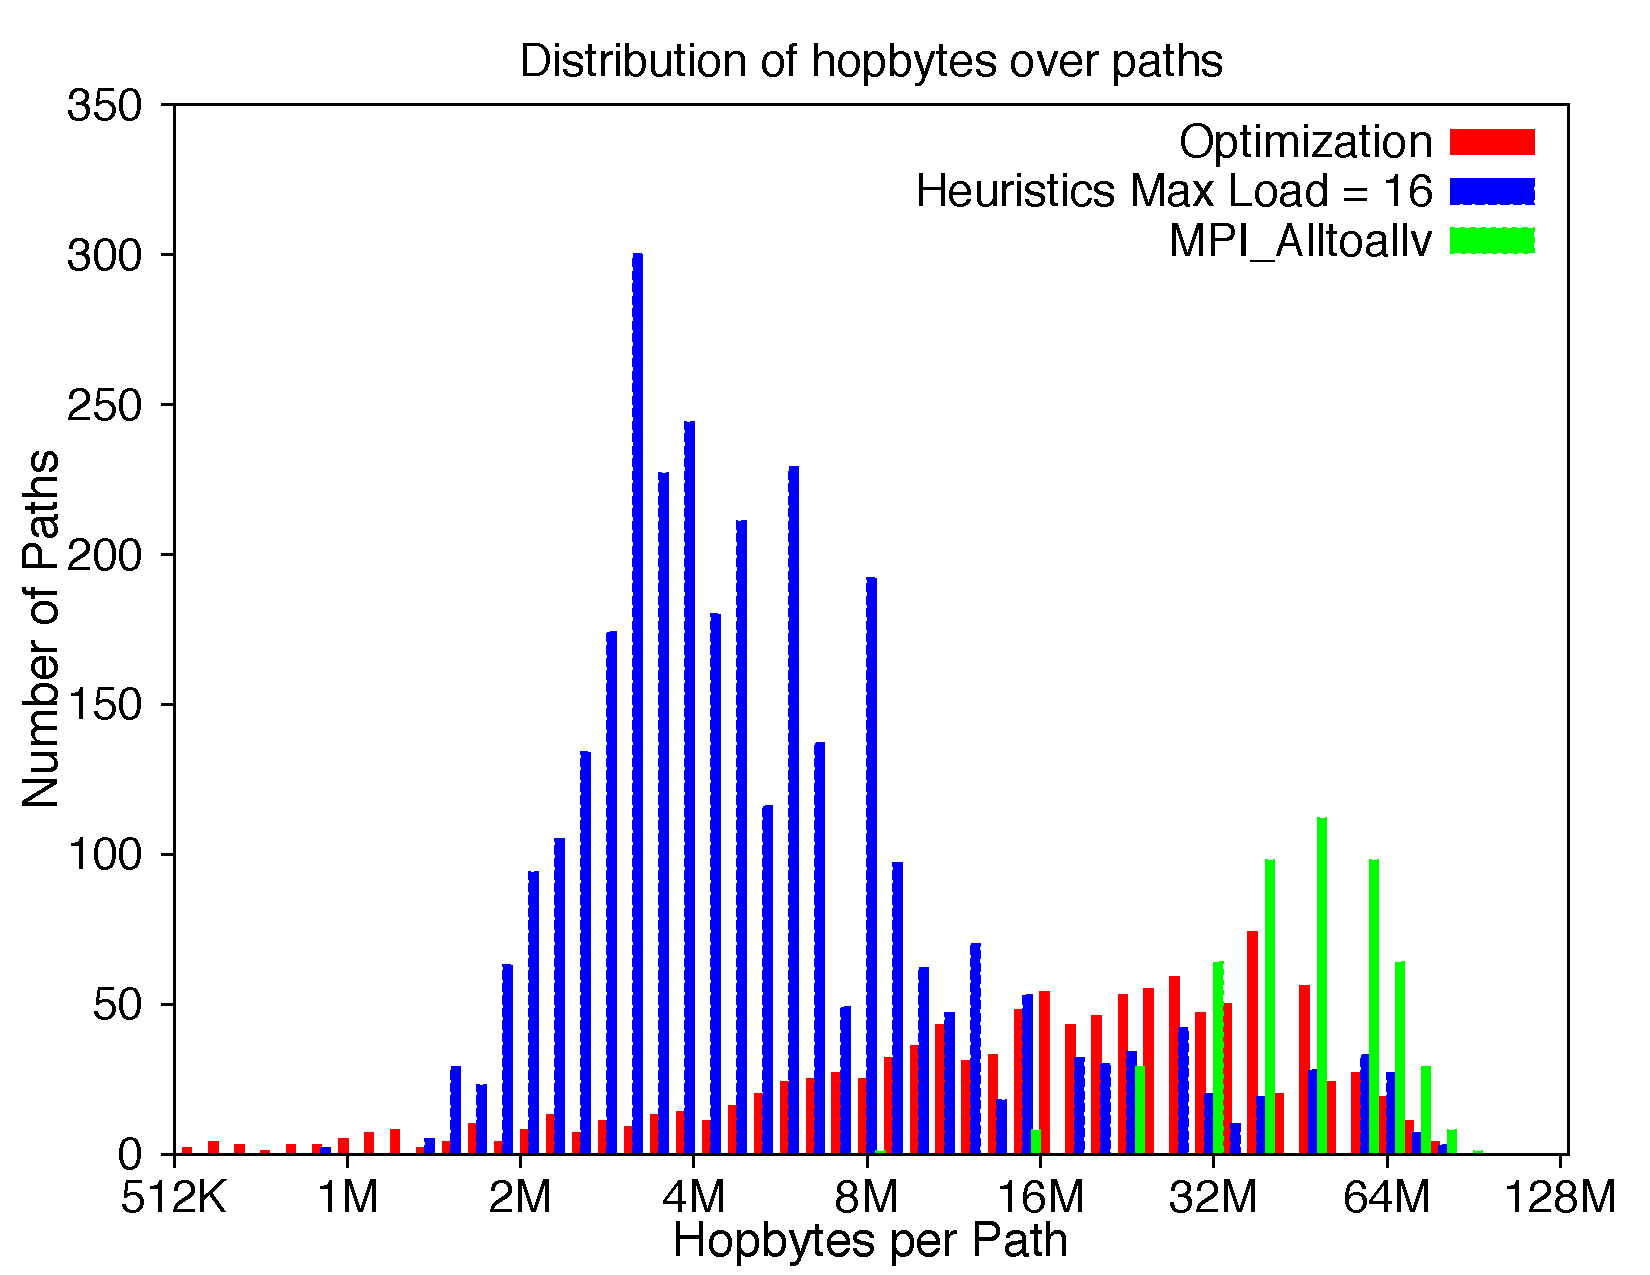
\includegraphics[scale=0.30]{figures/hopbyte_histo.pdf}
%\vspace{-0.1in}
%\caption{Distribution of hopbytes per path for Disjoint pattern in 1024-node partition.}
%\vspace{-0.1in}
%\label{fig:hopbyte_histo}
%\end{figure}


